\documentclass[a4j,fleqn,dvipdfmx,uplatex]{jsarticle}

\usepackage{sice-si}

\usepackage{epic,eepic}
\usepackage[dvipdfmx]{graphics}
\usepackage[dvipdfmx]{graphicx}
\usepackage[dvipdfmx]{color}
% \usepackage{fancyhdr} % ヘッダフッタの罫線と文字出力
% \pagestyle{fancy} % ヘッダフッタの罫線と文字出力(fancyhdrパッケージとセット)
\usepackage{amsmath} % 数式用
\usepackage{amssymb}
\usepackage{tabularx}
\usepackage{enumerate}
\usepackage{txfonts}
\usepackage{url}
\usepackage{pdflscape}
% \usepackage{bm}
\usepackage[subrefformat=parens]{subcaption}
\captionsetup{compatibility=false}

% 図表参照に章番号付加 章をまたいでの参照は不可
\newcommand{\figref}[1]{Fig.\ \ref{#1}}
\newcommand{\tableref}[1]{Table.\ \ref{#1}}

% 章番号の後調整
\newcommand{\secref}[1]{Section \ref{#1}\hspace{0.2zw}}
% 節番号の後調整
\newcommand{\subsecref}[1]{\ref{#1}\hspace{0.2zw} 節}


\begin{document}
%
% タイトルと著者名
\title{FTE新入社員課題報告書\\[1.5mm]本社屋上室外機における散水システム導入と\\省エネ効果に対する実験的検証} % 和文タイトル
\name{○高橋 京佑, 小坂 丞, 仲野 茂翠, 設樂 日和, 𠮷岡 拓海, 渡辺 夏芽, 
\\中村 天音, 塚田 浩貴, 青木 昇, 吉川 唯希, 佐藤 央都, 阪田 悠} % 著者名

\etitle{Introduction and Experimental verification on its energy-saving effect \\of Watering System for Condensing Unit on the office rooftop} % 英文タイトル
\ename{\small○KEISUKE Takahashi, TASUKU Kosaka, MOTOAKI Nakano, HINOWA Shidara, TAKUMI Yoshioka, NATSUME Watanabe, \\
AMANE Nakamura, HIROTAKA Tsukada, NOBORU Aoki, ITSUKI Yoshikawa, HIROTO Sato, YU Sakata}	%著者名(英)
%%%%%%%%%%%%%%%%%%%%%%%%%%%%%%%%%%%%%%%%%%%%%%%%%%%%%%%%%%%%%%%%%%%%%%%%%%%%%%%%%%%%%%%%%%%%%%%%%%%
% アブストラクト
\abst{}

% タイトルの出力
\maketitle
%%%%%%%%%%%%%%%%%%%%%%%%%%%%%%%%%%%%%%%%%%%%%%%%%%%%%%%%%%%%%%%%%%%%%%%%%%%%%%%%%%%%%%%%%%%%%%%%%%%
% 本文
\section{序論}\label{sec1}
\subsection{背景}\label{background}
近年, 地球温暖化の影響のため, 日本全国の気温は上昇傾向にあり, 
2021年の大阪府の年間平均気温は1883年に比べ2.5℃上昇している\cite{temp_osaka}. 
さらに, 2021年の真夏日と猛暑日の合計日数は, 2014年の65日に比べ13日増加, 
猛暑日に関しては8日増加しており\cite{temp_osaka2}, 1880年からの真夏日および
猛暑日の長期的推移を見ると増加傾向である (\figref{fig1:temp_osaka}). 

\begin{figure}[htb]
  \centering
  \begin{minipage}[b]{\linewidth}
      \centering
      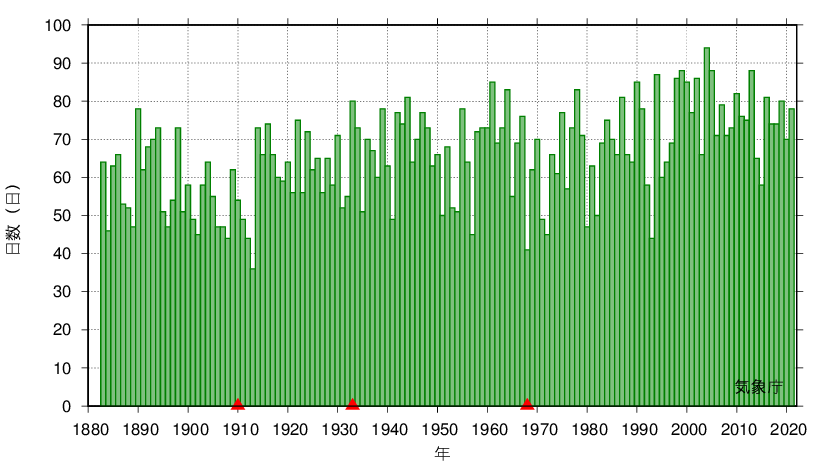
\includegraphics[width=\linewidth]{img/OSAKA_tmaxGE30.png}
      \subcaption{大阪 真夏日}
      \label{subfig1:temp_osaka}
    \end{minipage}\\
    \begin{minipage}[b]{\linewidth}
      \centering
      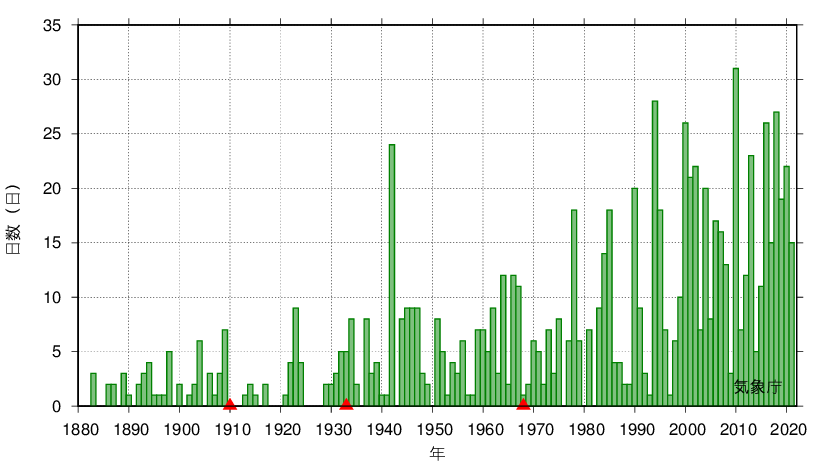
\includegraphics[width=\linewidth]{img/OSAKA_tmaxGE35.png}
      \subcaption{大阪 猛暑日}
      \label{subfig1:temp_osaka2}
    \end{minipage}
    \caption{真夏日および猛暑日の年間日数 1883-2021年\cite{temp_osaka3}}
    \label{fig1:temp_osaka}
\end{figure}
 
気温上昇に伴う問題点として, 空調による電力量の増加が懸念される. 
一般に空調機器は室内機と室外機に構成されており, 
冷房時において, 室外機は冷媒の圧縮・凝縮, 室内機は蒸発・膨張の過程をそれぞれ担っている. 
室外機は高圧化した冷媒ガスを外気と熱交換させることで凝縮させ, 
室内機では, 膨張した冷媒液を室内の空気と熱交換させて冷媒の潜熱を利用して冷却する. 

ここで, 室外機吸い込み側空気, つまり外気の温度が上昇すると, それに付随して凝縮温度
が高くなる. それにより凝縮負荷が大きくなり, 圧縮機の駆動力が占める比率が大きくなるため, 
結果的に成績係数が小さくなる. したがって, 同じ冷却能力を出すためには消費電力が大きくなる.  
さらに, 空冷機の冷却温度は外気温度マイナス10$^\circ$Cが目安とされており, 猛暑日になると
室内が十分に冷えなくなる可能性や高圧化防止のため運転が停止される問題もある. 

これらの問題を防止するために凝縮器の熱交換促進技術が様々考えられており, 特に
自動散水機の導入が挙げられる. 過去に散水装置を導入した食品メーカーの経済効果試算では
使用電力量は約7\%, 電気料金は約13\%の削減率が見込める結果となっている\cite{thesis3}. 

そこで, 実際に散水効果を検証するため, 室外機凝縮器部分にバケツを用いて散水をし, 
その電力量を計測した. 計測は本社2階北側のユニットクーラー用の室外機1台を用い, 
散水の有無による電力量の比較を行った. その際の計測環境は\tableref{table:ex1}に示す. 
\figref{fig1:compare_watering}に示すように, 実験2 (散水あり) の電力量は実験1 (散水なし) のそれと
比較して小さくなっていることが分かる.

\begin{table}[htb]
  \caption{計測環境}
  \label{table:ex1}
  \centering
  \begin{tabular}{lcccc}
     & 外気温 & 湿度 & 設定温度 & 気候 \\[-1.5mm]
     & [$^\circ$C] & [\%] & [$^\circ$C] &  \\
    \hline \hline
    実験1 & 34.3 & 48.0 & 27.0 & 晴れ  \\
    実験2 & 32.9 & 58.9 & 27.0 & 曇り \\
    \hline
  \end{tabular}
\end{table}

\begin{figure*}[htb]
  \centering
      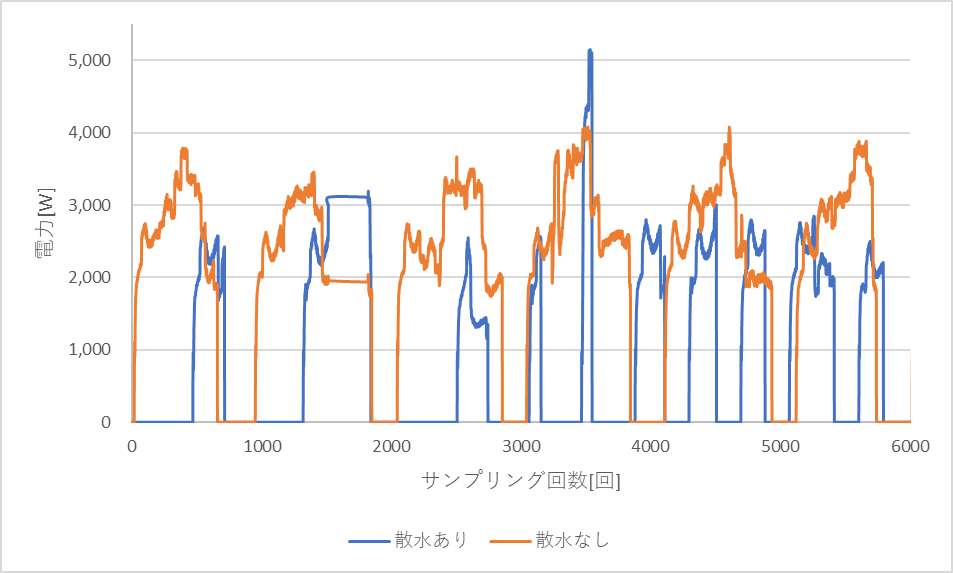
\includegraphics[width=0.8\linewidth]{img/ex1.png}
      \caption{散水の有無による電力量の比較}
      \label{fig1:compare_watering}
\end{figure*}


\subsection{目的}\label{purpose}
\subsecref{background} より, 室外機において散水装置の導入が電力量低減の効果
があるのではないかと考えられる. 
そこで本研究では, 散水システムの導入に伴い自作の散水装置を組み上げ, 
天候や室内設定温度など様々な条件下で比較検証を行い, 
電気代および水道代とのコストバランスを考慮に入れ, 最適な散水条件を検討することを
目的として実験を行った. 

\section{調査内容}\label{sec2}
本章では本研究で行った計測のための調査内容について説明する. 

本研究で調査対象とした室外機はビル用マルチエアコンである三菱社 
PUHY-EP335DMG9\cite{condensing_unit}を採用した (\figref{fig:condensing_unit}, \tableref{table:hard}). 
この室外機に散水の有無など, 以下の4条件に分けて計測を行っていく.  

\begin{description}
  \item[  実験1.1 ] 散水なし
  \item[  実験1.2 ] 散水あり (手動)
  \item[  実験1.3 ] 散水あり (自作)
  \item[  実験1.4 ] 散水なし (雨天)
\end{description}

\begin{figure}[htb]
  \centering
  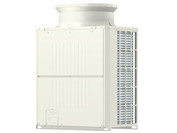
\includegraphics[width=0.7\linewidth]{img/PUHY-EP335DMG9.jpg}
  \caption{室外機 PUHY-EP355DMG9}
  \label{fig:condensing_unit}
\end{figure}

\begin{table}[htb]
  \caption{室外機仕様(冷房時)}
  \label{table:hard}
  \centering
  \begin{tabular}{lr}
    PUHY-EP355DMG9 & \\
    \hline \hline
    電源 & 3相 200V \\
    能力 & 33.5 kW \\
    消費電力 & 10.7 kW \\
    冷媒 & R410 \\
    \hline
  \end{tabular}
\end{table}



また、計測時間は日中で最も気温が高くなる13時から15時までの2時間とし, 
データログを取れるもの以外のパラメータは10分ごとに計測するとした. 


\subsection{自作散水システム}
本節では, 計測実験の比較対象として自作する散水システムの概要について説明する. 
屋上にある蛇口からホースと塩化ビニル管を結合させて室外機まで通し, 散水ノズルを
凝縮器側に左右3個ずつ計6個を設置した(\figref{fig2:watering_sys}). 

\begin{figure}[htb]
  \centering
    \begin{minipage}[b]{0.45\linewidth}
      \centering
      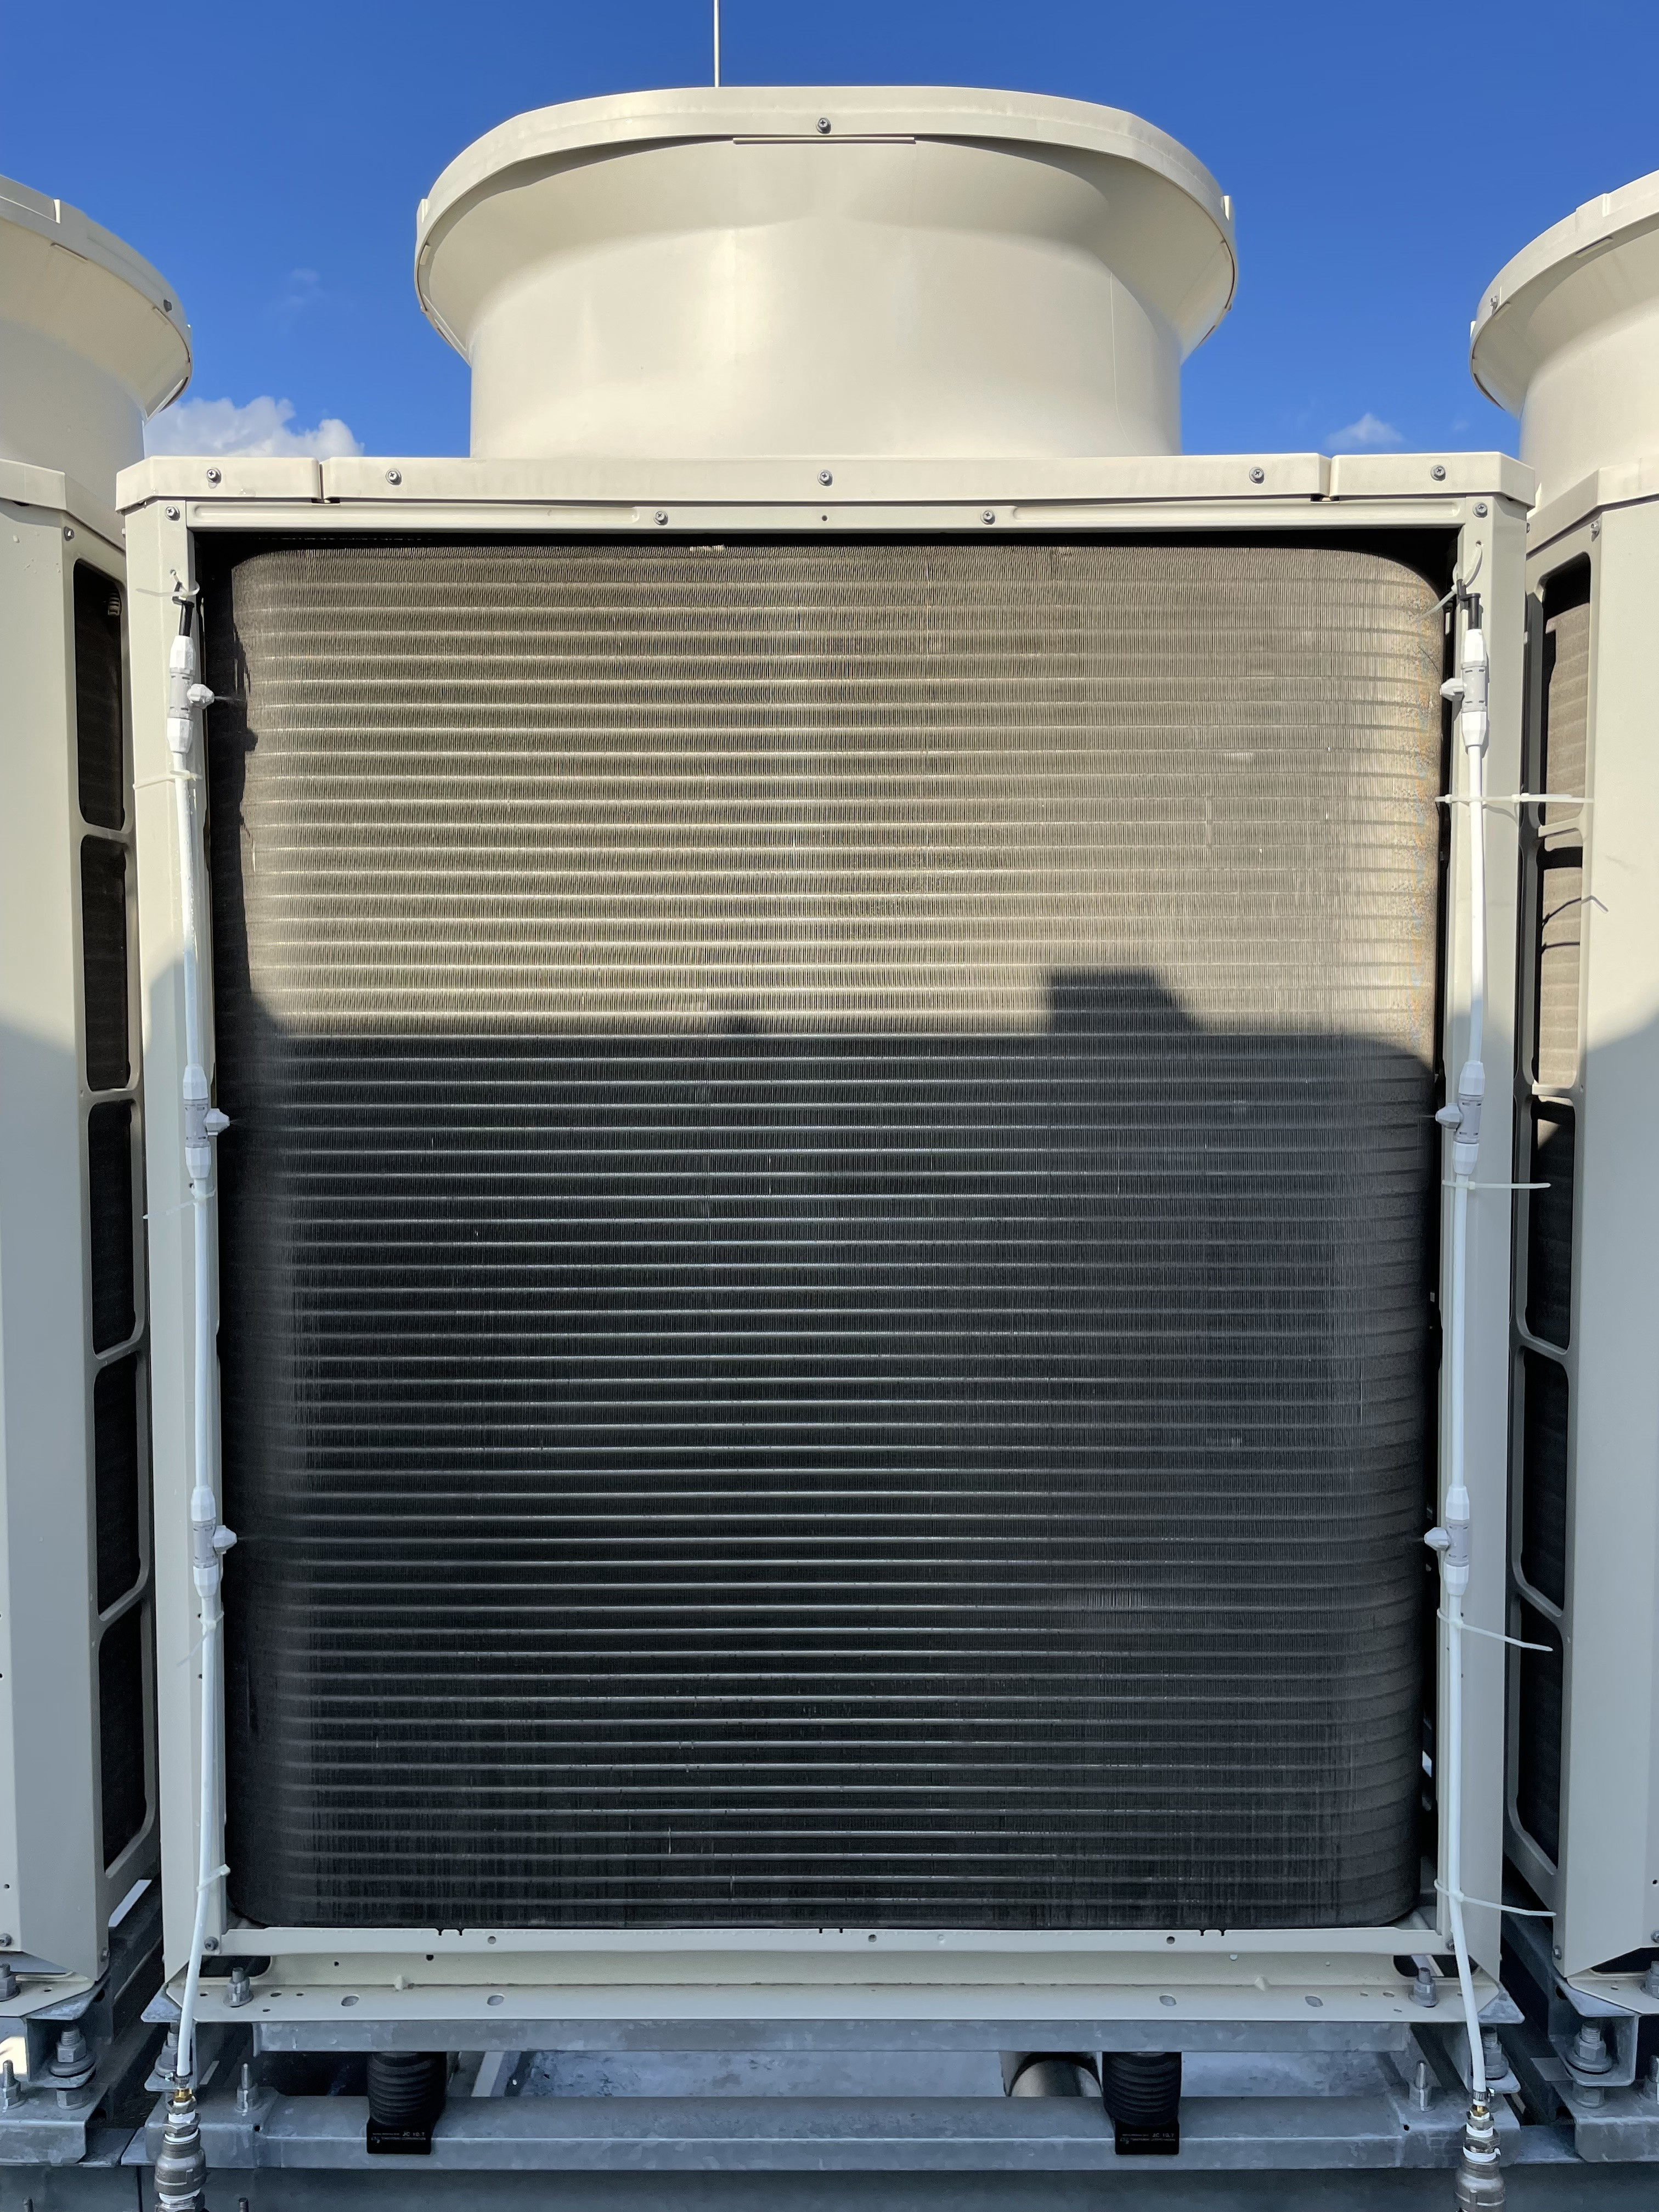
\includegraphics[width=\linewidth]{img/IMG_0146.jpg}
      \subcaption{凝縮器側}
    \end{minipage}
    \begin{minipage}[b]{0.45\linewidth}
      \centering
      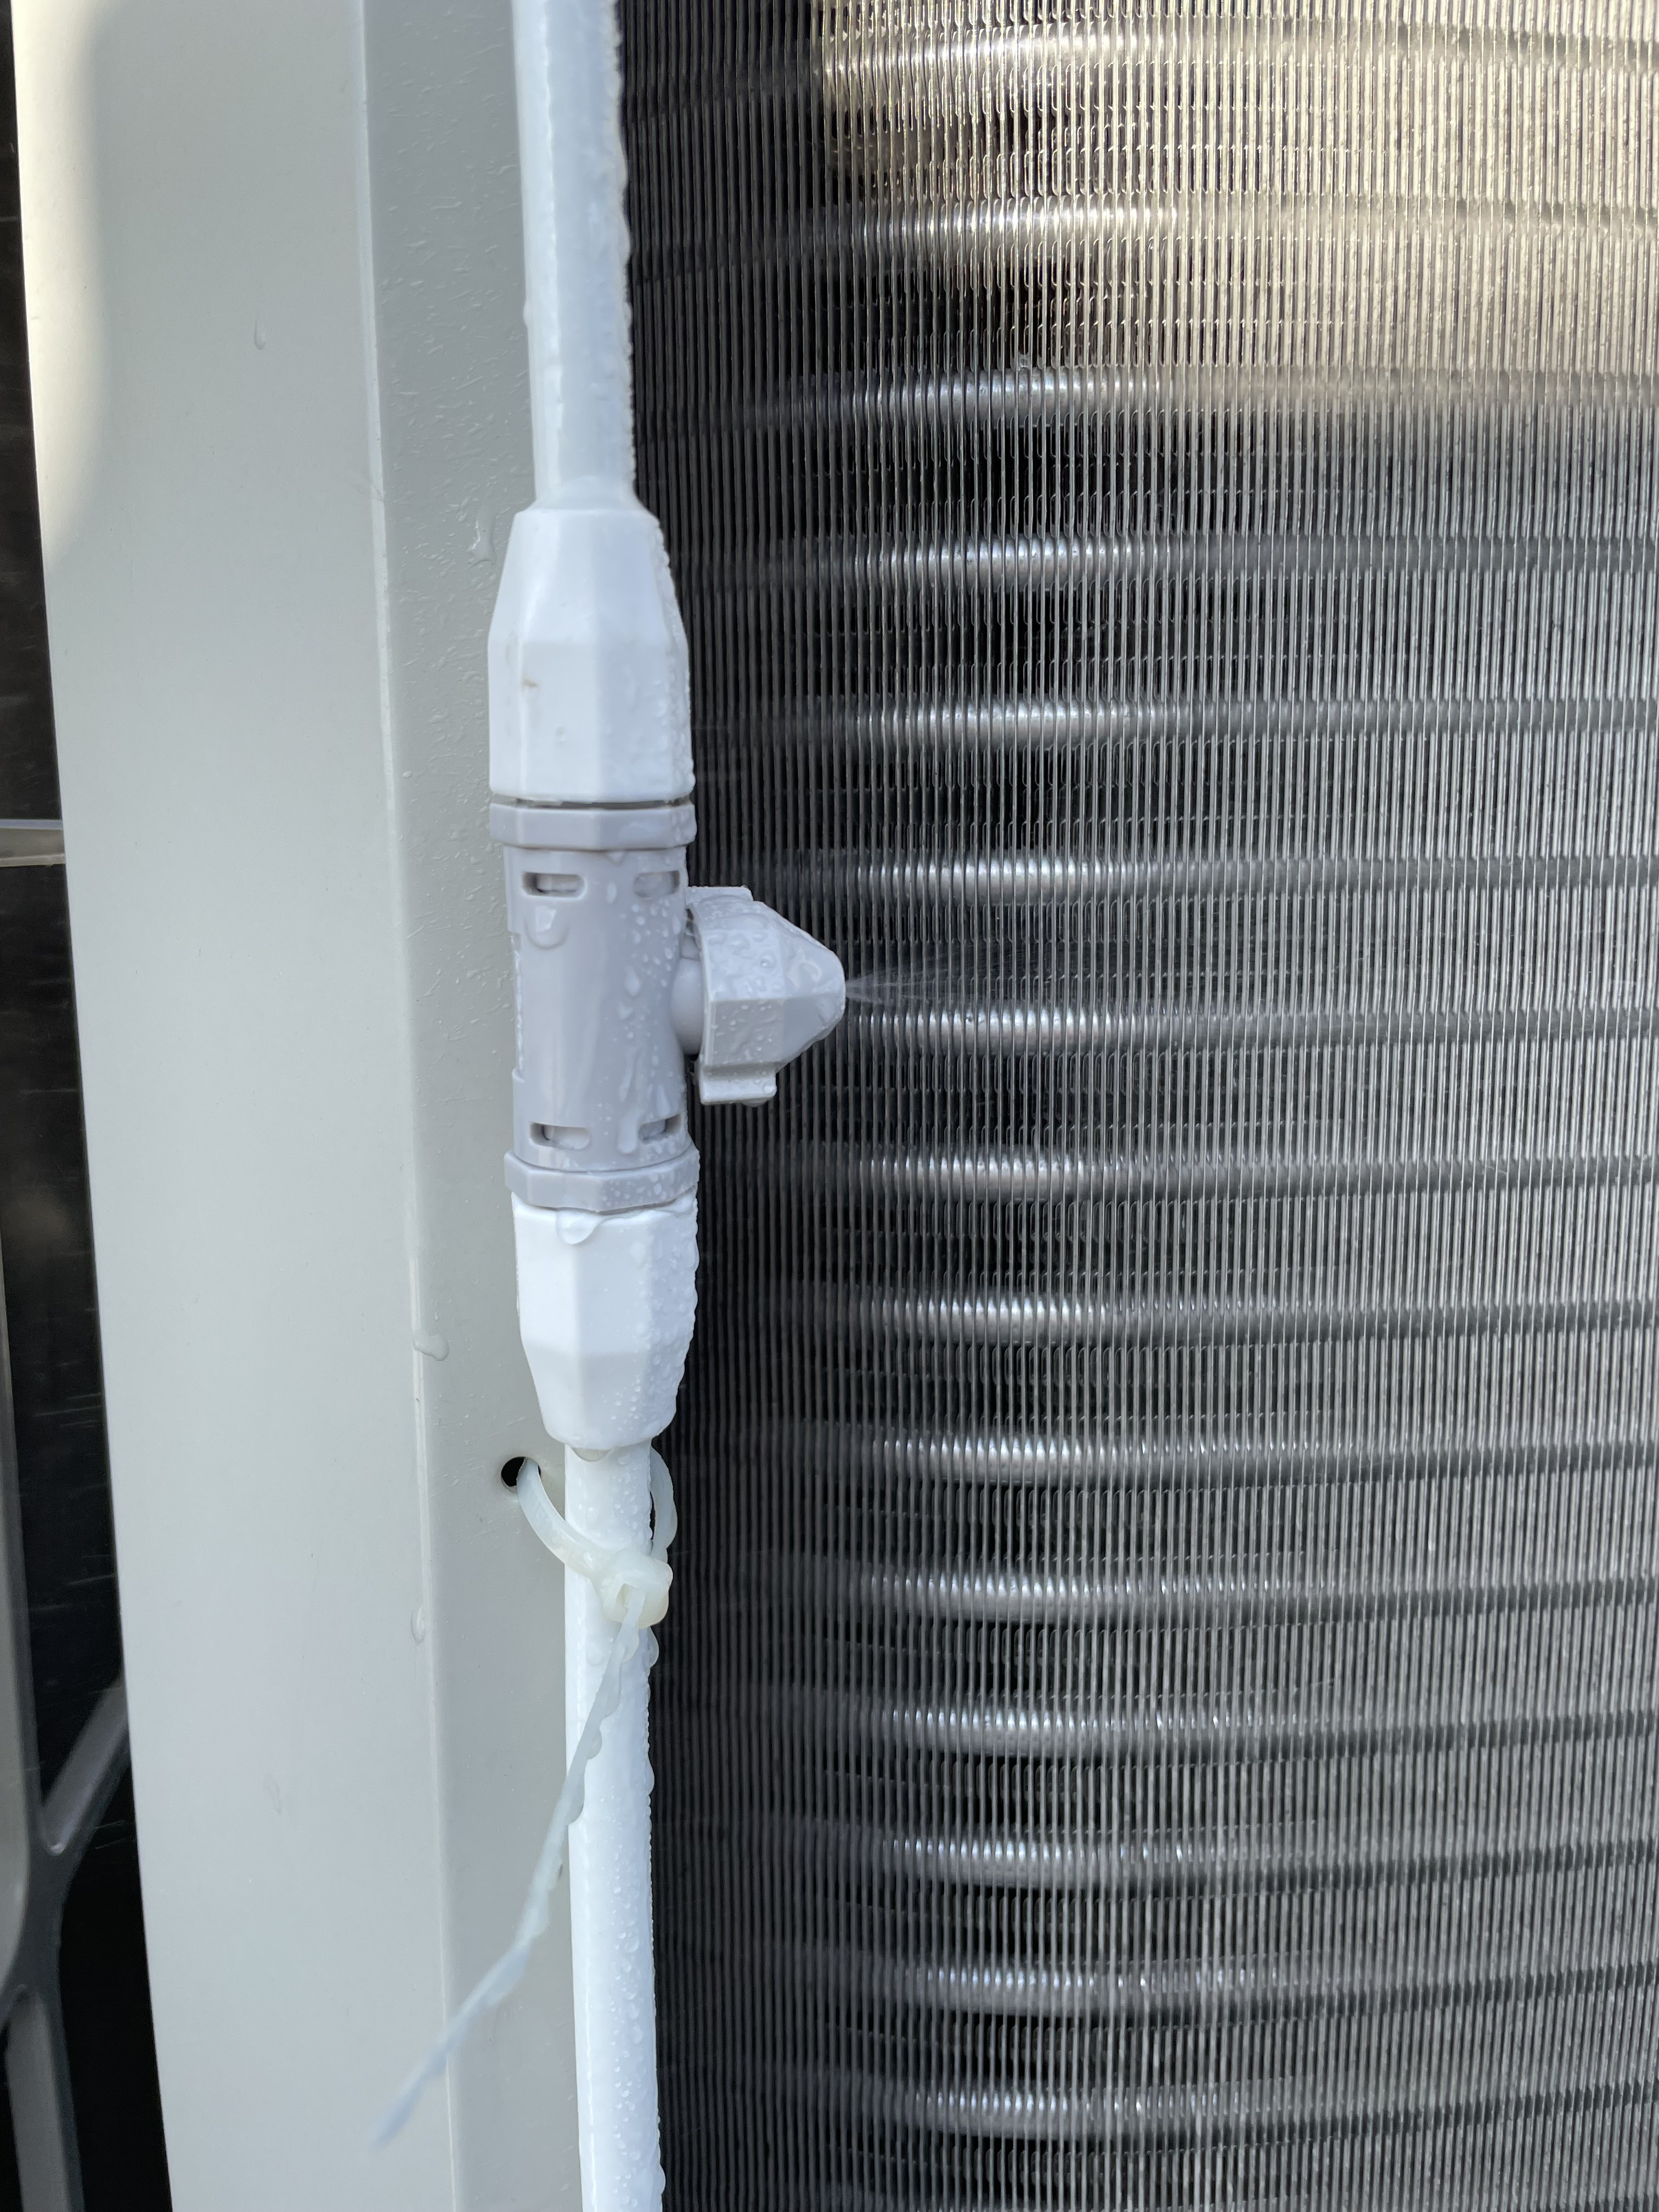
\includegraphics[width=\linewidth]{img/IMG_0142.jpg}
      \subcaption{散水用ノズル}
    \end{minipage}
  \caption{散水システム}
  \label{fig2:watering_sys}
\end{figure}

\begin{figure}[htb]
  \centering
  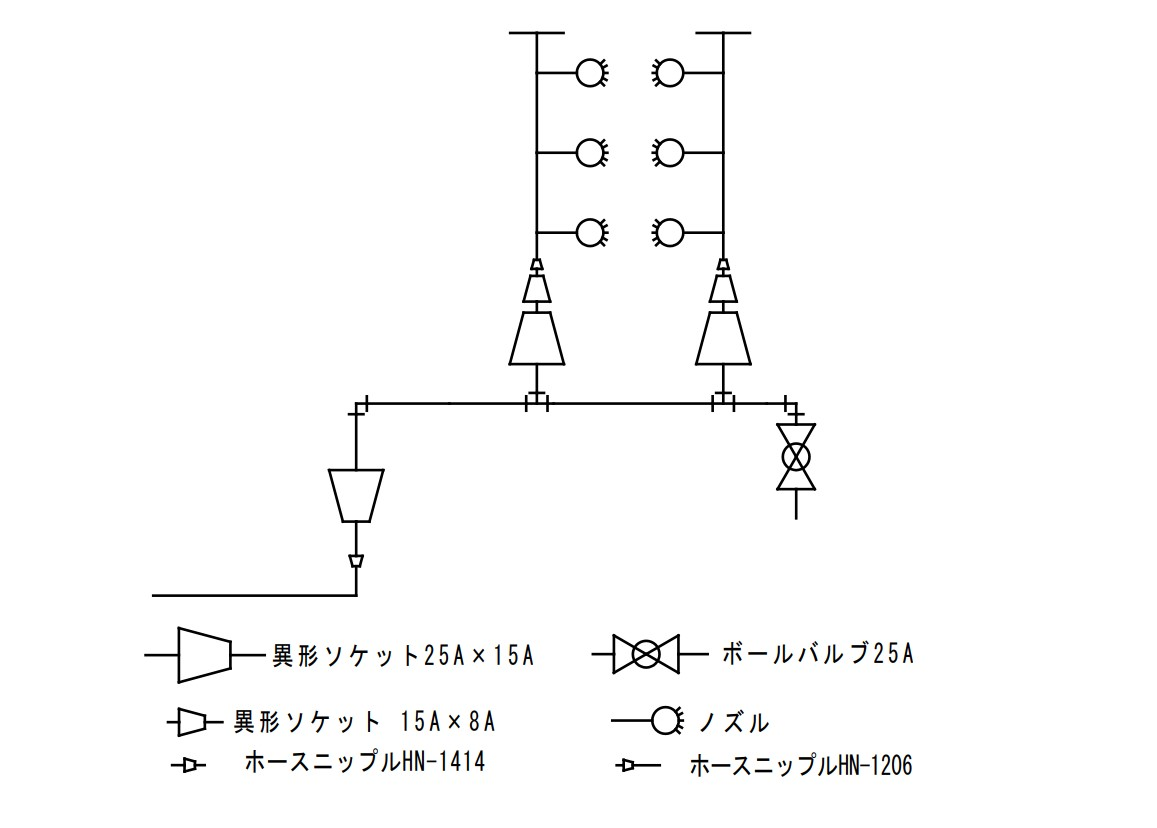
\includegraphics[width=\linewidth]{img/flow.jpg}
  \caption{自作散水システムの系統図}
  \label{fig:w_s_flow}
\end{figure}

\subsection{計測内容}
実験で計測するパラメータは以下の通りである. 

\begin{itemize}
  \item 外気環境(気温, 相対湿度, 風速)
  \item 凝縮器入口温度 (2箇所)
  \item 凝縮器出口温度 (2箇所)
  \item 室外機 (圧縮機運転状況)
  \item 電気系 (電流, 電圧, 電力量)
  \item 散水系 (水温, 散水流量)
  \item 室内系 (設定温度, 温湿度)
\end{itemize}

これらのパラメータを各実験で比較, 得られた電力量の差について考察していく. 

\section{結果}\label{sec3}
各条件での計測結果は\tableref{table:ex}に示す通りである. 

\begin{table}[htb]
  \caption{実験の計測環境及び結果}
  \label{table:ex}
  \centering
  \begin{tabular}{lrrrr}
    \small 計測日 & \small 気温 & \small 湿度 & \small 気候 & \small 設定温度 \\[-1.5mm]
     & \small [$^\circ$C] & \small [\%] & & \small [$^\circ$C] \\
    \hline \hline
    7/13 & 34.3 & 48.0 & 晴れ & 26 - 27 \\
    7/15 & 32.9 & 58.9 & 曇り & 27.0 \\
    7/19 & 27.9 & 82.8 & 雨 & 27.0 \\
    7/23 & 33.2 & 43.4 & 晴れ & 27.0 \\
    7/21 & 32.1 & 58.4 & 曇り/雨 & 27.0 \\[2.5mm]
    7/25 & 36.5 & 42.2 & 晴れ & 25.0 \\
    7/26 & 37.5 & 41.0 & 晴れ & 25.0 \\
    7/29 &  &  & 晴れ & 25.0 \\
    \hline
  \end{tabular}
\end{table}

\begin{table}[htb]
  \caption{2時間あたりの電力量およびその他比較指標}
  \label{table:ex2}
  \centering
  \begin{tabular}{lrrrrr}
    \small 計測日 &   \small 外気h & \small 消費電力 & \small 電気代 & \small 変化率\\[-1.5mm]
    & \small [kJ/kg] & \small [kWh] & \small [円] & \small [\%] \\
    \hline \hline
    27℃ \\
    \hline
    7/13 & 76.5 & 4.24 & 118 & ― \\
    7/15 & 80.9 & 1.66 & 42 & 35.6 \\
    7/19 & 78.4 & 2.88 & 72 & 61.0 \\
    7/23 & 66.2 & 0.72 & 18 & 15.3 \\
    7/21 & 77.5 & 1.04 & 26 & 22.0 \\[2mm]
    25℃ \\
    \hline
    7/25 & 78.5 & 3.12 & 80 & ― \\
    7/26 & 80.6 & 4.45 & 112  & 140 \\
    7/29 &  &  &   &  \\
    \hline
  \end{tabular}\\
  ※ h : 比エンタルピー
\end{table}

\begin{figure}[htb]
  \centering
  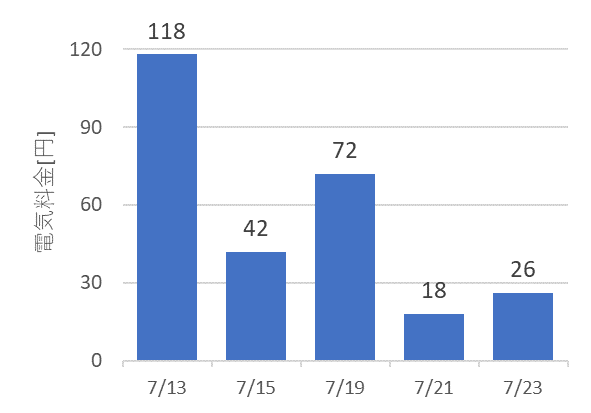
\includegraphics[width=0.8\linewidth]{img/fee_27.png}
  \caption{電気料金比較 (実験グループ1)}
  \label{fig:fee_27}
\end{figure}

各計測実験での電力量との推移は\figref{fig1:compare_watering}に示す. 

従量電気料金を25円として見積もった際の各実験における2時間でかかった電力量
および電気代は\tableref{table:ex2}および\figref{fig:fee_27}に示す. 


% 仮挿入
\begin{figure*}[htb]
  \centering
  \begin{subfigure}[b]{0.42\linewidth}
    \centering
    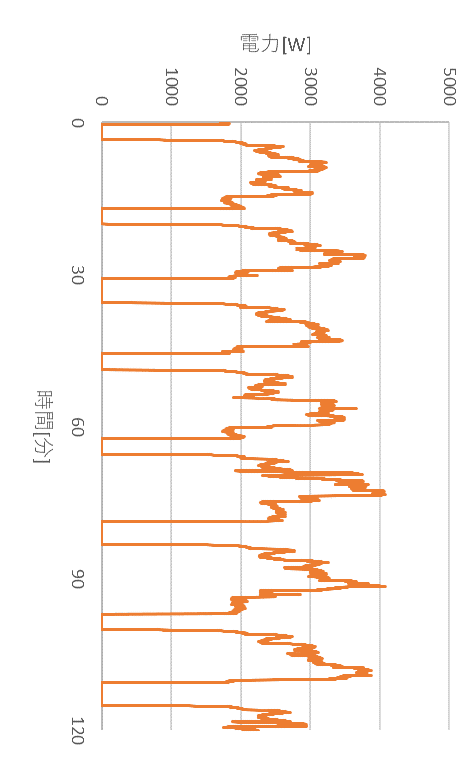
\includegraphics[width=\linewidth]{img/0713_power.png}
    \caption{7/13(27℃ 散水なし)}
  \end{subfigure}
  \begin{subfigure}[b]{0.42\linewidth}
    \centering
    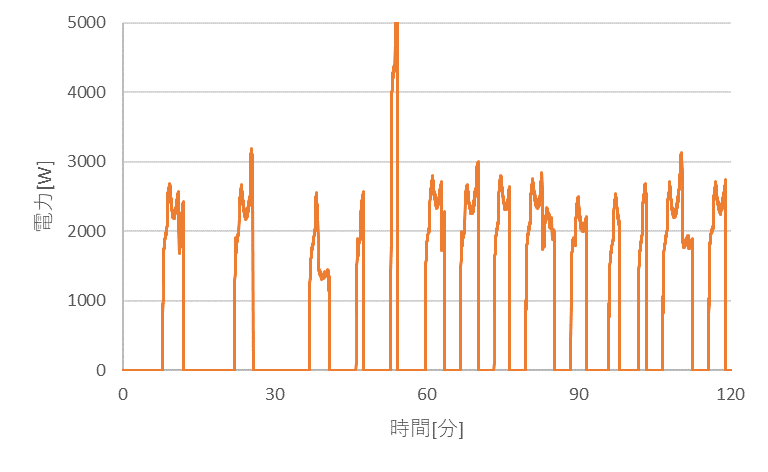
\includegraphics[width=\linewidth]{img/0715_power.png}
    \caption{7/15(27℃ 手動散水)}
  \end{subfigure}\\
  \begin{subfigure}[b]{0.42\linewidth}
    \centering
    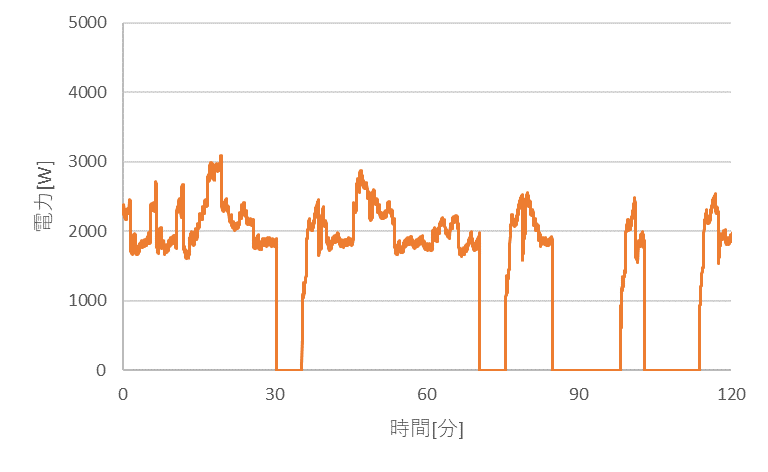
\includegraphics[width=\linewidth]{img/0719_power.png}
    \caption{7/19(27℃ 雨天)}
  \end{subfigure}
  \begin{subfigure}[b]{0.42\linewidth}
    \centering
    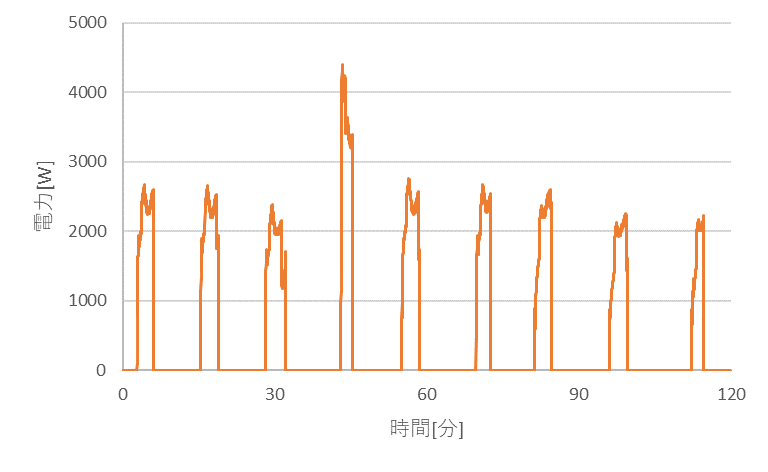
\includegraphics[width=\linewidth]{img/0721_power.png}
    \caption{7/21(27℃ 手動散水)}
  \end{subfigure}
  \caption{電力量推移と散水タイミング(1 of 3)}\label{fig2:ex_outputs_1/3}
\end{figure*}

\begin{figure*}[htb]
  \addtocounter{figure}{-1}
  \centering
  \begin{subfigure}[b]{0.4\hsize}
    \addtocounter{subfigure}{4} % 最初のsubfigure数 15を加える
    \centering
    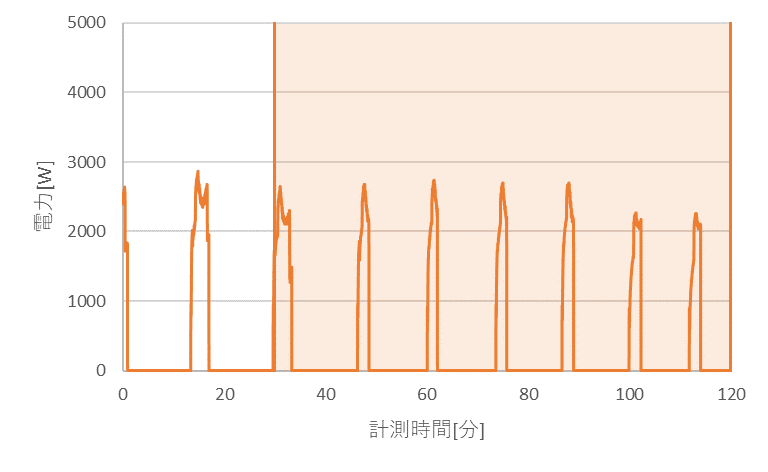
\includegraphics[width=\linewidth]{img/t_p/20220723.png}
    \caption{7/23(27℃ 手動散水)}
  \end{subfigure}
  \begin{subfigure}[b]{0.4\hsize}
      \centering
      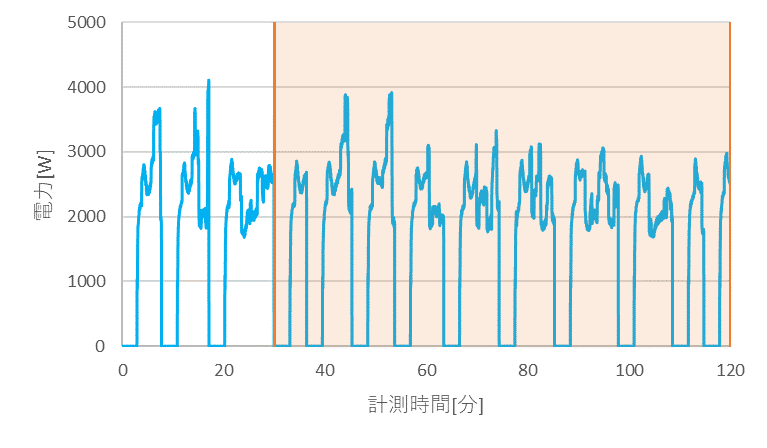
\includegraphics[width=\linewidth]{img/t_p/20220725.png}
      \caption{7/25(25℃ 散水なし)}
  \end{subfigure}\\
  \begin{subfigure}[b]{0.4\hsize}
      \centering
      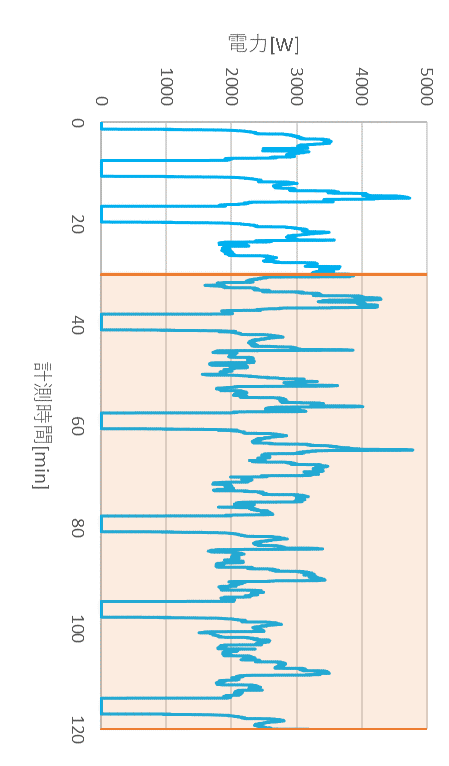
\includegraphics[width=\linewidth]{img/t_p/20220726.png}
      \caption{7/26(25℃ 自動散水)}
  \end{subfigure}
  \begin{subfigure}[b]{0.4\hsize}
      \centering
      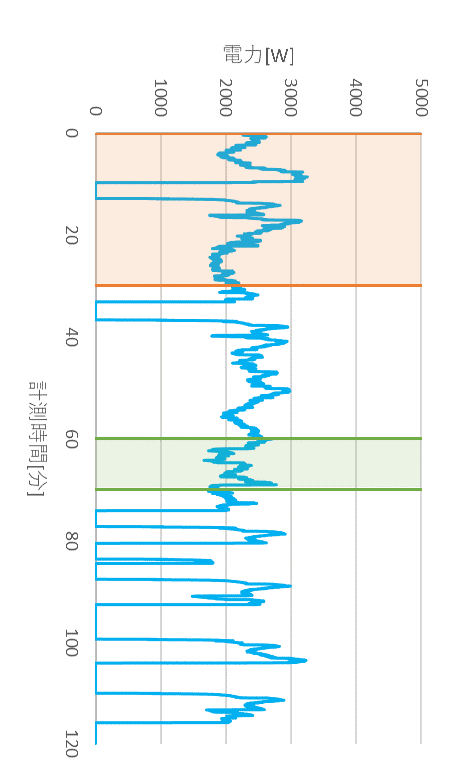
\includegraphics[width=\linewidth]{img/t_p/20220728.png}
      \caption{7/28(25℃ 自動散水)}
  \end{subfigure}
  \caption{電力量推移と散水タイミング(2 of 3)\\背景色付きは継続散水を表す}\label{fig2:ex_outputs_2/3}
\end{figure*}

\begin{figure*}[htb]
  \addtocounter{figure}{-1}
  \centering
  \begin{subfigure}[b]{0.4\linewidth}
    \addtocounter{subfigure}{8} % 最初のsubfigure数
    \centering
    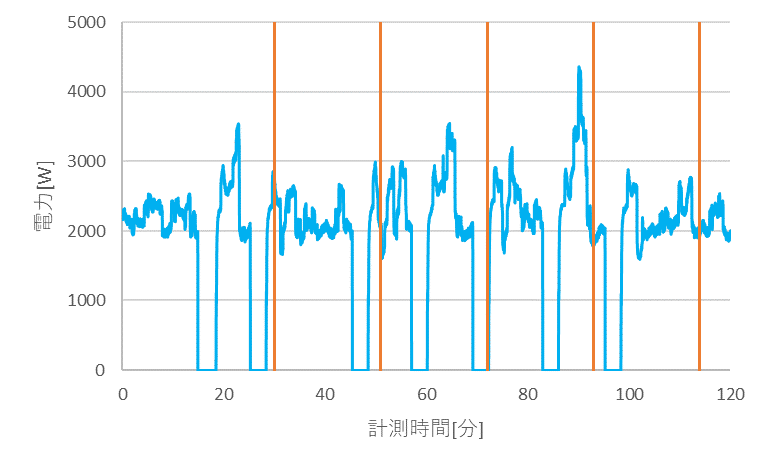
\includegraphics[width=\linewidth]{img/t_p/20220729.png}
    \caption{7/29(25℃ 自動散水)}
  \end{subfigure}
  \begin{subfigure}[b]{0.4\linewidth}
    \centering
    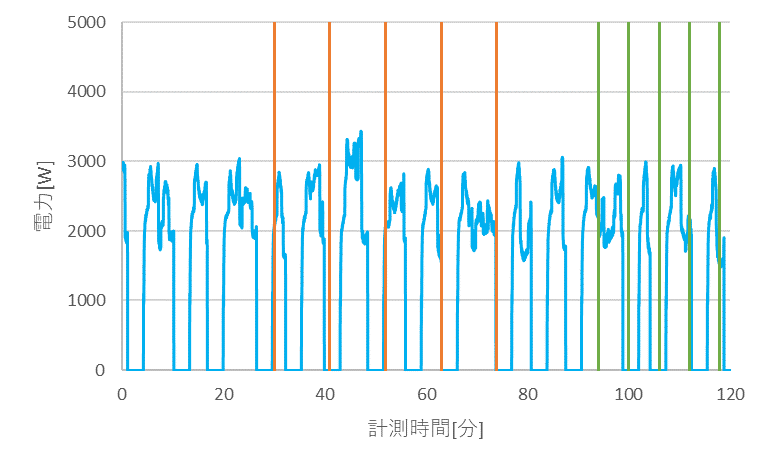
\includegraphics[width=\linewidth]{img/t_p/20220803.png}
    \caption{8/3(25℃ 自動散水)}
  \end{subfigure}
  \caption{電力量推移と散水タイミング(3 of 3)}\label{fig2:ex_outputs_3/3}
\end{figure*}


\section{考察}\label{sec4}
(挿入したグラフ)に示す通り, 散水した場合は最大消費電力および運転時間が
小さくなっている事が分かる. 
\figref{fig:fee_27}から, 実験1に比べた消費電力の減少率は, 実験2で約60\%, 
実験4で約32\% 減少することが分かった. 
これらの値は外気環境が異なるため, 正当性の評価としては難しい面があるが, 大まかな比較として
電力量が減少していることが分かる. 

また, 散水ありの場合でも, 手動で行った場合と自動機器を用いて散水した場合では
〇〇\% 減少率に偏差が生まれた. これは散水量と散水範囲の違いも考慮できるが, 
大部分は, 紙コップで散水したのに対し, ノズルによる散水は粒子の大きさが小さいために
水の潜熱による凝縮器吸込温度の低下が効率良く行えたことによるものが大きいと考えられる. 
今回手動の散水では約〇〇Lの水を1分間かけて散水するのを2回行ったが, 十分効果があるため, 
機器の導入が難しい場合であっても有効な手段であると考える. 
しかし, 散水は炎天下のなか行う場合が多いため, 担当者の負担と人的コストと考慮すると賢明な
判断とは言い難い. 

本州などの比較的平均気温の高い地域では, 導入におけるイニシャルコストは
約〇〇ヶ月で償却できるであろう. 



\subsection{グラフによる考察}
に示すように散水を停止した時間に好成績を収めている. これはフィンに付着した水滴
が蒸発した潜熱によるもの、或いはファンが吸い込んだ内側の水滴が蒸発したためであると考察する. 
ここで, 1分間の散水量は約450mlであり

一見, 一貫性がなく見えるが散水タイミングと圧縮機の運転ピークの始まりと終わりのタイミングに
相関あるように見受けられる. これは散水タイミングと合わせると潜熱を使い切った状態である. 


\section{結論と今後の課題}
本章では計測結果および\secref{sec4}からの考察を総括した結論を示す. 

雨天時や長時間散水の計測結果から, 継続的な散水はフィンに水滴が付着することにより熱交換が阻害されることがわかった. 
また, 水滴の蒸発速度はその半径に概ね比例する. 
これらのことから, 散水時間を断続的にする, 散水粒子の半径を小さくする, 散水角度など
による散水方法の工夫が必要である. 
また, 散水時間を短くすると蒸発速度が速くなるので散水回数の考慮が必要であるが, 
今回の計測装置の条件では15分に1回程度が適正であった. 

\subsection{今後の課題}
\cite{thesis3} スケール対策

%参考文献
\begin{thebibliography}{99}
\bibitem{temp_osaka}
国土交通省, 気象庁, 大阪府 日最高気温の月平均値, 
\url{https://www.data.jma.go.jp/obd/stats/etrn/view/monthly_s3.php?prec_no=62&block_no=47772&year=&month=&day=&view=a2}\vspace{2mm}

\bibitem{temp_osaka2}
George's Web Sites, 大阪府-大阪市の気温に関する統計情報, 
\url{http://www.tvg.ne.jp/george/weather/gw_stat_temp.html?city=oosaka}\vspace{2mm}

\bibitem{temp_osaka3}
A-PLAT 気候変動適応プラットフォーム, 気候変動の観測・予測データ, 大阪府観測データ, 
\url{https://adaptation-platform.nies.go.jp/map/Osaka/index_past.html}\vspace{2mm}

\bibitem{condensing_unit}
三菱電機, 暮らしと設備の業務サイト WIN2K, ビル用マルチエアコン 室外ユニット PUHY-EP335DMG9, 
\url{https://www.mitsubishielectric.co.jp/ldg/wink/ssl/displayProduct.do?pid=317186&ccd=2020121158}\vspace{2mm}

% \bibitem{clie}
% 株式会社クリエ, 高圧カット防止室外機散水装置 トラブルカット, 
% \url{https://c-clie.shop-pro.jp/?pid=134166927}\vspace{2mm}

% \bibitem{daisen}
% ダイセン・メンブレン・ システムズ株式会社, 
% 室外機向け散水システム "E mizu Shower System", 
% \url{https://daicen.com/products/kankyo/emizushower.html}\vspace{2mm}

\bibitem{thesis2}
"エアコン室外機への散水による省エネ効果の実験結果", 
総合技術センター計測・制御技術分野 飯田 仁\vspace{2mm}

\bibitem{夏の節電}
資源エネルギー庁, "2.夏の節電生活の基本を知っておく"\vspace{2mm}

\bibitem{thesis3}
"空調室外機散水システム(Eミズシャワー)による節電・CO2 削減", 
綿部智一, 中塚修志, 
ダイセン・メンブレン・システムズ株式会社技術開発センター\vspace{2mm}

\end{thebibliography}
%
%
%
\end{document}